\chapter{Development}
\section{Initial testing}
\subsection{Storing questions - Regex}
One of the features that the program requires is an ability to generate random questions. An initial idea was to just store the questions in a text file.
\begin{figure}[H]
	\centering
	\texttt{A ball is projected with speed 20 ms$^{-1}$. At the starting point the ball is 12m of the ground. The highest point of the ball is 20m. Find theta.}
	\caption{Initial question store}
\end{figure} 
The problem with this method is that it is hard to randomise the question. This is because the parts to be randomised in the string are not easily identifiable. 
\begin{figure}[H]
	\centering
	\texttt{A ball is projected with speed [speed]. At the starting point the ball is [height] of the ground. The highest point of the ball is [highpoint]. Find theta.} 
	\caption{Question store with identifiable variables}
\end{figure}
Now the variables can be differentiated from other text, this allows a regular expression to be constructed. The regular expression  will return text enclosed by brackets.
\begin{figure}[H]
	\texttt{import re\\
		question = "A ball is projected with speed [speed]."\\
		variables = re.findall(r'\textbackslash [\textbackslash w+\textbackslash ]', question)\\
		print(variable)\\
		>>> ['[speed]']}
	\caption{Extracting variables from a string using Python regex}
\end{figure} 
This shows how the variables could be extracted using python code. A random number could then be inserted using \texttt{random.randint(range)} function. 

There are downsides to using regular expressions. While it is easy to generalise areas of the string that you would like to capture, the expression can get very complex and hard to maintain. I don't think that I have sufficient experience in using regular expressions to be able to confidently use them in this project, so this method was discarded.
\subsection{Storing questions - String formatting}
Python has built in methods to format strings. This is shown in Figure 2.3 found in Section 2.5.4. This functionality is quite basic, and does not allow you to extract the name of the identifiable variable stored in the string (Figure 3.2). This means that it is hard to extract the name of the variable.

Fortunately there is a way to extend the functionality of the inbuilt Python string formatter, so that it can be customised to your needs. More details about that can be found in PEP 3101\autocite{pep3101}. This shows that you can create a class, that takes a string as an input, and formats the text however you would like it to. 

\begin{figure}[H]
\begin{lstlisting}[language=Python,]
	class object:
	  def __format__(self, format_spec):
	    return format(str(self), format_spec)
\end{lstlisting}
\caption{Example of extended string formatting\autocite{pep3101}}
\end{figure}

This shows how much you can custom the string formatter. An example string for use in this is shown in Figure 2.4.

This method was chosen for use in the project.

\subsection{Graph generation}
There are many Python libraries that allow you to plot graphs and draw diagrams. The most popular library is Matplotlib, which was initially created in 2002 by John Hunter. It allows data to be plotted in a highly customisable way, and interacts very well with Python arrays, which is useful when the data being plotted is generated at runtime.

\begin{figure}[H]
	\centering
	\begin{lstlisting}[language=Python]
	import matplotlib.pyplot as plt
	plt.plot([1,2,3,4])
	plt.ylabel('some numbers')
	plt.show()
	\end{lstlisting}
	
	\caption{Code to create Figure 3.6 \autocite{mpl}}
\end{figure}
This is code used to generate the simple graph seen below.
\begin{figure}[H]
	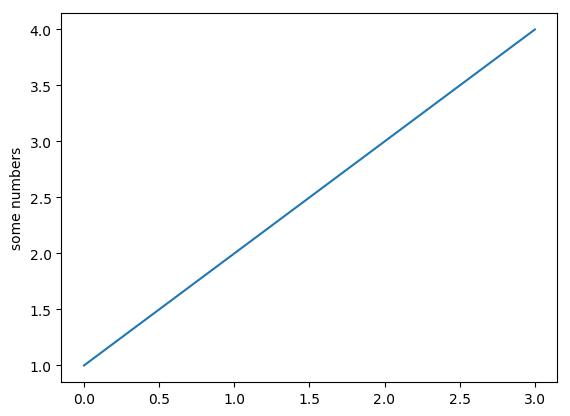
\includegraphics[width=\textwidth,height=\textheight,keepaspectratio]{exmpl.png}
	\caption{Graph generated by code in Figure 3.5}
\end{figure}
The code in Figure 3.5 shows how easy it is to draw a clean looking graph, which would be suitable for use in the program.

Other Python plotting libraries were not looked at, as Matplotlib is perfect for the needs of the project. It is also part of the Anaconda platform\autocite{conda} which is a Python installation containing many scientific Python libraries.  This library was chosen for use in the project.

\subsection{GUI}
There are hundreds of libraries to display GUI's in Python, but there are three that are most commonly used which are:
\begin{itemize}
	\item Tkinter
	\item PyQT
	\item WxPython
\end{itemize}
These are all Python wrappers for C/C++ code, which can make development hard because in some cases error codes may not be returned to the Python console, so you don't know what you have done wrong.

WxPython was immediately discounted, as it does not have stable support for Python version 3.x .

Next tkinter was considered. tkinter is a Python wrapper of Tcl/tk. It is class based, so to create a GUI you must create a class that extends the base frame class, and to customise this frame, you must override methods from the parent class. While the code is not that complex itself, the positioning of elements can get very complex, as it must be done entirely in code, as there is no WYSIWYG\footnote{What you see is what you get.} editor. As this project has a time constraint, tkinter was discarded.

Lastly PyQt was looked at. PyQt is a Python wrapper for Qt, which is a highly popular GUI framework, which is even used for the main touchscreen in the Tesla Model S. Qt comes with an excellent WYSIWYG editor, allowing you to easily create a GUI without having to worry about the code behind it. The code generated however is in C, which would be hard to integrate with the other Python code.

Luckily, there is a program called PyUIC5, which converts C code used to display a Qt GUI, into Python code that performs exactly the same function. This is the perfect tool for this project, as it allows the GUI to be created easily, and functionality to be easily added to the buttons, by extending some classes in the Python code.

Here is how the GUI design workflow will work with PyQt:
\begin{enumerate}
	\item Design GUI in QtCreator
	\item Convert generated C code into Python
	\item Add functionality to buttons in Python code
\end{enumerate}

PyQt was chosen as the GUI tool.

\subsection{Summary}
\begin{itemize}
	\item Extending the Python string formatter for storing questions
	\item Matplotlib for drawing the graphs
	\item PyQt for displaying the GUI
\end{itemize}
\section{Storing questions}
I decided to code each element of the program separately, and then once they are working on their own, to integrate them into the final project. I started writing the question store code first, as it just used vanilla Python, so I didn't have to worry about trying to install libraries. 

The code for overriding the Python string formatter was implemented first.
\begin{lstlisting}[language=Python, caption=Formatter override]
#RandomizedFormatter class. Child of Randomized class. Overrides String formatter to allow
#question formatting.
class RandomizedFormatter(object):
	def __init__(self, name, args):
		self.name = name
		self.args = args

	#This function overrides the Python string formatter.
	def __format__(self, fmt):
		op, rest = fmt.split(':', 1)
		
		if op == 'type':
			self.args[self.name] = rest
			return ""
		elif op == 'random':
			low, high = rest.split(':')
			value = random.randint(int(low), int(high))
			self.args[self.name] = value
			return str(value)
\end{lstlisting}
This piece of code overrides the Python string formatter. It then formats the question with this algorithm:
\begin{itemize}
	\item Find text enclosed by curly braces and place into a list.
	\item Split the text at the colons.
	\item Determine what the operator is.
	\item Format the text according to the operator.
	\item Store the randomized variable.
\end{itemize}
The operators available are \texttt{type}, and \texttt{random}. If the operator is type, then in the questionstore file the variable will look like this \texttt{\{equation:type:equationtype\}}. This allows the program to know which equation to use with the data it is given.

For the \texttt{random} operator, the variable will look like this \texttt{a:random:5:30} where \texttt{a} is the name of the variable that the random value will be stored in, \texttt{random} is the operator, and \texttt{5:30} is the range for the random number generation. 

Now that the code for formatting the string is complete, it was decided to create a parent class which would have other methods. This class would have to be able to return the answer to the question, the values of the randomly generated variables, and also the formatted string. This is the first version of the code for this.
\begin{lstlisting}[language=Python, caption=questionStore Parent Class v1]
class Randomized(object):
	def __init__(self):
		self.args = {}
		self.question = None
	
	#Returns the value of the randomized variable in the string.
	def __getitem__(self, name):
		return RandomizedFormatter(name, self.args)
	
	#Formats the string, using the overridden method found in the RandomizedFormatter class.
	def format(self, s):
		return string.Formatter().vformat(s, args=(), kwargs=self)
	
	#Returns the question class depending on the equation type.
	def get_class(self):
		if self.args['equation'] == "findtheta":
			self.question = questionplotclass.ProjectileQuestion(self.args['b'], self.args['a'], random.randint(40, 60))
			answer = self.question.answer_theta()
			return answer
		if self.args['equation'] == "findmaxheight":
			self.question = questionplotclass.ProjectileQuestion(self.args['c'], self.args['a'], self.args['b'])
			answer = self.question.answer_max_height()
			return answer
		if self.args['equation'] == 'findxdistance':
			self.question = questionplotclass.ProjectileQuestion(self.args['c'], self.args['a'], self.args['b'])
			answer = self.question.answer_xdistance
			return answer
\end{lstlisting}
This code couldn't be properly tested, as the \texttt{questionPlotClass} hadn't been written yet, so random numbers were given as answers for testing. While this code returns the answer, there is a problem because when the class is initialised, a random number is used, and this is not stored. This means that if another method wants to be called on the class, it will most likely have a different result, as the random number generated will be different.

This problem was solved by instead of just returning the answer, the instance of the class was returned. This meant that any method could be called on this instance of the class, without having to store the random number. 

A function was also added to retrieve a random line from a text file of questions. This is the \texttt{load} 
The second version of the \texttt{get\_class} function:
\begin{lstlisting}[language=Python, caption=Second iteration of the get\_class function]
#Returns the question class depending on the equation type.
def get_class(self):
	if self.args['equation'] == "findtheta":
		self.question = questionplotclass.ProjectileQuestion(self.args['b'], self.args['a'], random.randint(40, 60))
		self.question.find_theta()
		return self.question
	if self.args['equation'] == "findmaxheight":
		self.question = questionplotclass.ProjectileQuestion(self.args['c'], self.args['a'], self.args['b'])
		self.question.find_max_height()
		return self.question
	if self.args['equation'] == 'findxdistance':
		self.question = questionplotclass.ProjectileQuestion(self.args['c'], self.args['a'], self.args['b'])
		self.question.find_xdistance()
		return self.question
\end{lstlisting}
You can see that this code now returns the instance of the class instead of the answer.

Now that both the parent and child class were complete, they were put together to make the final Python file for the question formatting.
\lstinputlisting[language=Python, caption=Final questionStore code]{../questionStore.py}
Here is a list of features that this piece of code performs:
\begin{itemize}
	\item Formats a question string by replacing variables with random numbers and storing value.
	\item Allows the instance of the class used to display the question to be returned so other methods can be called on it.
	\item Loads a random question string from a text file.
\end{itemize} 
\section{Graph Generation}
After the code for string formatting was completed, next the code for the graph generation was made. This code is linked to the question generation, as it requires the random variables, and the equations used to generate the graph can also be used to create an answer.
\subsection{Equations}
To generate the graphs, a series of coordinates that the particle will pass through need to be calculated. matplotlib will then draw a smooth curve between these points. To keep things simple, and similar to the A2 Maths and Physics syllabus air resistance is ignored. So the horizontal speed won't change, and can be written as \[v_x = u\cos\theta\] where $u$ is the initial speed, and $\theta$ is the angle the particle is launched to the horizontal. The position can then be calculated by using distance = speed x time, so the equation for horizontal displacement is \[S_x = tu\cos\theta\]

The vertical position is a bit harder to calculate as gravity is being simulated. Luckily there is an equation of motion which is perfect for this scenario: \[S = ut + \frac{1}{2}at^2\] where $t$ is the time in seconds, and $a$ is the acceleration due to gravity. This equation needs to be tweaked slightly, as we need resolve the initial speed to find the vertical component. \[v_y = u\sin\theta\]
We can then put this into the equation of motion
\[S_y = ut\sin\theta  + \frac{1}{2}at^2\] 

Now that we have equations for both the x and y displacement, we can generate of list of coordinates using an algorithm like this:
\begin{algorithm}
	\caption{Coordinate list generation}
	\begin{algorithmic}[1]
		\For{i in range 0, upperBound}
			\State tempPos = []
			\State tempPos.append($iu\cos\theta$)
			\State tempPos.append($S_y = ui\sin\theta  + \frac{1}{2}ai^2$)
			\State coordinateArray.append(tempPos)
		\EndFor
	\end{algorithmic}
\end{algorithm}
Now that we have the pseudocode, this loop needs to be implemented in Python.
\begin{lstlisting}[language=Python, caption=Coordinate generation loop]
while (yPosTemp > 0): #While the particle is above the ground
	xPosTemp = xSpeed * time
	yPosTemp = (ySpeed * time) + (0.5 * -9.8 * time ** 2)
	xPos.append(xSpeed * time)
	yPos.append((ySpeed * time) + (0.5 * -9.8 * time ** 2))
	time += increment
\end{lstlisting} 
For this code I used a separate array for the x position and the y position, but that should not matter at this stage. A while loop is used in this case, as I want the graph to only show up to when it hits the ground again after being fired, so the while loop keeps generating coordinates until it is below the ground.

\subsection{Graph drawing}
Using the list of coordinates generated using the code above, we can use matplotlib to display the graph. I started from the bottom, so a simple graph was made first. 
\begin{lstlisting}[language=Python, caption=First graph generation code]
import matplotlib.pyplot as plt
import numpy as np

increment = 0.0001  # Time increment used when calculating values
initialSpeed = 10
theta = np.radians(70)  # Angle that the direction of launch makes to the horizontal
xSpeed = initialSpeed * np.cos(theta)  # Using trig to calculate xspeed. Assumes there is no air resistance
ySpeed = initialSpeed * np.sin(theta)
xOffset = 0  # Initial x position. Can be changed to add an offset which can be in a question
yOffset = 0  # Initial y position. Can be changed to add an offset which can be in a question
xPos = []  # X position array
yPos = []  # Y position array
time = 0  # Initial time

xPos.append(xOffset)  # Adding the offset in the first slot of the position array
yPos.append(yOffset)  # Adding the offset in the first slot of the position array

time += increment

xPosTemp = xSpeed * time  # Calculating first x value so while loop doesn't fail instantly
yPosTemp = (ySpeed * time) + (
0.5 * -9.8 * time ** 2)  # Using SUVAT to calculate first y value. This is so that the while loop doesn't fail instantly
xPos.append(xPosTemp)
yPos.append(yPosTemp)

while (yPosTemp > 0):
	xPosTemp = xSpeed * time
	yPosTemp = (ySpeed * time) + (0.5 * -9.8 * time ** 2)
	xPos.append(xSpeed * time)
	yPos.append((ySpeed * time) + (0.5 * -9.8 * time ** 2))
	time += increment

plt.plot(xPos, yPos)
plt.axis([0, xPos[len(xPos) - 1], 0, max(yPos)])
plt.xlabel("X displacement")
plt.ylabel("Y displacement")
plt.show()
\end{lstlisting}
This generates
\begin{figure}[H]
	\centering
	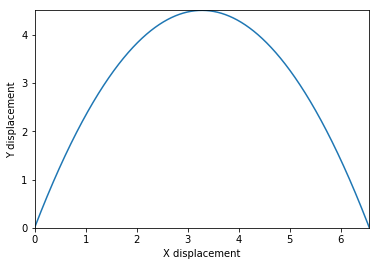
\includegraphics[width=\textwidth,height=\textheight,keepaspectratio]{firstgraph.png}
	\caption{First graph}
\end{figure}
This is perfectly acceptable graph, although it is a bit boring, and the y axis is a bit small, as the top of the graph is cut off slightly. This can be easily fixed by changing line 36 in Listing 3.6 to 
\lstinline[language=Python] $ plt.axis([0, xPos[len(xPos) - 1], 0, max(yPos) + max(yPos) * .2])$. This will increase the height of the axis by the same amount, no matter the launch parameters of the particle, as it is being multiplied by a constant. 

At this point it was decided that questions generated using this graph would be too boring, and simple. So another type of question was chosen similar to this
\begin{figure}[H]
	\centering
	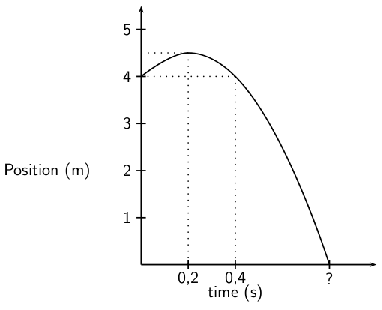
\includegraphics[width=\textwidth,height=\textheight,keepaspectratio]{graph2}
	\caption{Example of a graph \autocite{graph2}}
\end{figure}
This type of graph allows the initial height offset to be randomised, which can make for a more interesting question, and requires some more complex mathematics to solve.

The next generation of the graph was then coded, which meant that particle started at an offset above the ground. Labels were added for the maximum height, and the distance travelled before it hits the ground.
\begin{lstlisting}[language=Python, caption=Second iteration of graph generation]
import matplotlib.pyplot as plt
import numpy as np


def y_displacement(y_offset, initial_speed, theta):
	increment = 0.001
	theta = np.radians(theta)
	x_speed = initial_speed * np.cos(theta)
	y_speed = initial_speed * np.sin(theta)
	x_pos = []
	y_pos = []
	time = 0
	x_pos.append(0)
	
	y_pos.append(y_offset)  # Adding the offset in the first slot of the position array
	
	time += increment
	x_pos_temp = x_speed * time  # Calculating first x value so while loop doesn't fail instantly
	y_pos_temp = (y_speed * time) + (
	0.5 * -9.8 * time ** 2) + y_offset
	
	x_pos.append(x_pos_temp)
	y_pos.append(y_pos_temp)
	
	while y_pos_temp > 0:
		y_pos_temp = (y_speed * time) + (0.5 * -9.8 * time ** 2 + 12)
		x_pos.append(x_speed * time)
		y_pos.append((y_speed * time) + (0.5 * -9.8 * time ** 2) + 12)
		time += increment
		x_distance = max(x_pos)
	plt.plot(x_pos, y_pos)
	plt.annotate(s="", xy=(-1, y_offset), xytext=(-1, 0), arrowprops=dict(arrowstyle='<->'))
	plt.annotate(s="", xy=(0, -1), xytext=(max(x_pos), -1), arrowprops=dict(arrowstyle='<->'))
	plt.plot([0, x_distance], [0, 0], color='k', linestyle='-', linewidth=2)
	plt.plot([0, 0], [0, y_offset], color='k', linestyle='-', linewidth=2)
	plt.plot([-0, -1], [y_offset, y_offset], color='k', linestyle='-', linewidth=2)
	plt.plot([0, x_pos[y_pos.index(max(y_pos))]], [y_offset, y_offset], color='k', linestyle='--', linewidth=2)
	plt.annotate(s="", xy=(x_pos[y_pos.index(max(y_pos))], max(y_pos)),
	xytext=(x_pos[y_pos.index(max(y_pos))], y_offset), arrowprops=dict(arrowstyle='<->'))
	plt.text(-max(x_pos) * 0.08, y_offset / 2, str(y_offset), style='normal')
	plt.text(max(x_pos) / 2, -max(x_pos) * 0.05, str(max(x_pos)), style='normal')
	plt.text(x_pos[y_pos.index(max(y_pos))] + 1, ((max(y_pos) - y_offset) / 2) + y_offset, str(max(y_pos) - y_offset),
	style='normal')
	plt.axis([-5, x_distance, -5, max(y_pos) + 5])
	plt.axis('off')
	plt.show()

y_displacement(12, 20, 30)
\end{lstlisting} 
\begin{figure}[H]
	\centering
	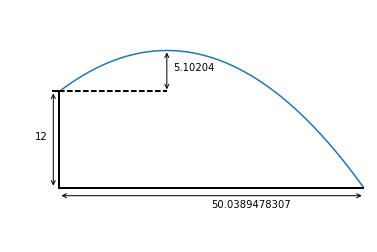
\includegraphics[width=\textwidth,height=\textheight,keepaspectratio]{graph3}
	\caption{Second iteration of graph}
\end{figure}
As you can see this graph is much more interesting that the previous graph. It shows the data needed to answer questions clearly, and it is easy to randomise the variables in it. 

Then questions needed to be designed around this style of graph, so I the questions will be either finding $\theta$, finding the maximum height or finding the distance travelled before it hits the ground. To display these without giving the answer away, I will have to not show some information on the graph depending on the type of question, and also add an indication of which angle $\theta$ is on the graph. 

First I added an arrow showing the initial launch. To draw an arrow you have to give the function two points. The first point was trivial, it was just (0, y offset) however the second point was more involved as it had to be at the right angle. I used trigonometry to work out this point, and the Python code is shown below.
\begin{lstlisting}[language=Python, caption=Arrow coordinate generator]
def calculate_point(start_x, start_y, angle, length):
	endpoint = [start_x + (length * np.cos(angle)), start_y + (length * np.sin(angle))]
	return endpoint
\end{lstlisting}
When you call the function it will return a list of the two coordinates. This can then be used to generate the arrow. This arrow was added with this line of code 
\lstinline[language=Python]|plt.annotate(s="", xy=(0, y_offset), xytext=(calculate_point(0, 12, theta, 10)), arrowprops=dict(arrowstyle='<-'))|
The graph now looks like this:
\insertimage{graph4}{Third iteration of graph}

Next $\theta$ needed to be displayed on the graph. There were three ways to do this, either to draw the symbol manually with a line and an eclipse, use an image of the symbol or use \LaTeX to generate the symbol. I decided to use \LaTeX as it meant that I could easily use other symbols if necessary. 

"LaTeX, which is pronounced «Lah-tech» or «Lay-tech» (to rhyme with «blech» or «Bertolt Brecht»), is a document preparation system for high-quality typesetting. It is most often used for medium-to-large technical or scientific documents but it can be used for almost any form of publishing."\autocite{latex}. This is also what I am using to create this document.

To use \LaTeX with Python is not trivial. You must first get a working installation of \LaTeX on your computer, which is usually done with MikTeX on a Windows machine. Then you must configure matplotlib to use \LaTeX which is done by adding the lines:
\begin{lstlisting}[language=Python, caption=Requirements for \LaTeX in matplotlib]
plt.rc('text', usetex=True) 
plt.rc('font', family='serif') 
\end{lstlisting}
Then to use \LaTeX to display math characters, you must precede the string with \texttt{r}. 
\begin{lstlisting}[language=Python, caption=String used to display $\theta$ using \LaTeX]
r'\textbf{\ensuremath{\theta}'
\end{lstlisting}
The symbol was then added to the graph with this line of code 
\lstinline[language=Python]|plt.text(0 + initial_speed * 0.09, y_offset + initial_speed * 0.02, r'\textbf{\ensuremath{\theta}') |
A label for the initial speed was also added.
\insertimage{graph5}{Fourth iteration of graph}

Finally the angle arc had to be drawn. This was done using Matplotlib patches, which were quite complex. They work essentially like stickers, where you create the item you would like to place, and then you place it at specific coordinates on the graph. The arc was create using this code
\begin{lstlisting}[language=Python, caption=Requirements for \LaTeX in matplotlib]
arc = patches.Arc((0, y_offset), 7, 7,
angle=0, theta1=360, theta2=30, linewidth=1)
\end{lstlisting}
This however is hard coded, so the arc will not change when the angle changes. This can be fixed by changing \lstinline|theta2=30| to \lstinline|theta2=np.degrees(theta)|.
\insertimage{graph6}{Final iteration of graph}
At this point I realised that I would not have enough time to complete the radioactive decay part of the questions, so I decided to focus on the projectile motion questions.

\subsection{Question class}
Once the graph generation was coded, this was put into a class to collect the methods together and make it easy to reuse. The Class created can be found in Algorithm 6 and 7 in Section 2.5
\section{GUI Design}
As mentioned before, Qt has a great GUI designer which I will use to create the GUI. Before the GUI was made in QT Creator, the design was prototyped.
\insertimage{hcl}{GUI Design Prototype}
Figure 3.13 is clear and functional. It has large title, so it is clear to the user which topic they are practising. 

Now that the prototype was made, the design was then created in Qt Creator. This program was slightly more difficult to use than expected, as the building was not truly drag and drop. A grid had to be created first, and then items put into it with spacers to change their position, otherwise the window just collapses on itself. This was discovered after the first prototype was created and it was then changed after that.
\insertimage{projmotioncreator}{Projectile motion screen in Qtcreator}
On the right hand side of the image, you can see a list of the components used to make up the screen. The parent component is the grid, which is used so that spacers can be placed, and so that elements will keep their shape. 

Looking at the main window, The blue squiggly lines are spacers. These are used to move elements around, as elements can not be dragged and dropped into position, as was found out in the initial test of the prototype.

The green boxes are the areas that contain a label, for example the title "Projectile motion questions". Labels are also used as a placeholder for the image, as there is not an image element. The label is then replaced by an image when the GUI is being prepared for display.

Buttons can also be seen on the screen, in the top left and at the bottom next to the answer text box. 

The answer text box at the bottom is a simple textbox to allow the user to enter their answer to the question.

\subsection{Porting GUI into Python}
Now that the GUI was created in Qtcreator, and the Qt code was automatically created by Qtcreator, the Qt code had to be converted into Python code so that the GUI could be interacted with in Python. 

Luckily this was not too hard as there is a command line tool called \texttt{pyuic}. This allows you to convert the Qt code into Python code with the command \texttt{pyuic -o file} where \texttt{file} is the filename that the Python code will be exported to. 

During the development stage, the GUI design was changed frequently, and it became tiresome having to run the \texttt{pyuic} command everytime a change was made. To solve this problem, a Windows \texttt{.bat} file was created so that the command did not have to be written out each time. 
\begin{lstlisting}[language=bash, caption=Batch script to update Python code]
IF EXIST C:\Users\TomEaton\PycharmProjects\school\projectilegui.py del /F C:\Users\TomEaton\PycharmProjects\school\projectilegui.py 

pyuic5 -o C:\Users\TomEaton\PycharmProjects\school\projectilegui.py C:\Users\TomEaton\Documents\suvat\suvat.ui
\end{lstlisting}
This script checks if \texttt{projectilegui.py} file already exists. This file contains the Python code generated by pyuic. If it does exist, it is deleted. This is because when \texttt{pyuic} writes to a file, it fails if the file already exists. The next line then runs the \texttt{pyuic} command detailed above.

The Python code generated is by no means the most optimal, but the performance gain from writing the code by hand would have minimal benefit compared to the time saved by having the code automatically generated.

\begin{lstlisting}[language=Python, caption=\texttt{PyQt} code generated by \texttt{pyuic}]
self.lineEdit.setObjectName("lineEdit")
self.gridLayout_2.addWidget(self.lineEdit, 1, 0, 1, 1)
self.pushButton_2 = QtWidgets.QPushButton(self.gridLayoutWidget_2)
self.pushButton_2.setObjectName("pushButton_2")
self.gridLayout_2.addWidget(self.pushButton_2, 1, 1, 1, 1)
self.label = QtWidgets.QLabel(self.gridLayoutWidget_2)
sizePolicy = QtWidgets.QSizePolicy(QtWidgets.QSizePolicy.Expanding, QtWidgets.QSizePolicy.Preferred)
sizePolicy.setHorizontalStretch(0)
sizePolicy.setVerticalStretch(0)
sizePolicy.setHeightForWidth(self.label.sizePolicy().hasHeightForWidth())
self.label.setSizePolicy(sizePolicy)
self.label.setMinimumSize(QtCore.QSize(500, 0))
self.label.setMaximumSize(QtCore.QSize(10000000, 16777215))
self.label.setObjectName("label")
self.gridLayout_2.addWidget(self.label, 0, 2, 2, 2)
\end{lstlisting}
This is an extract of the generated code. As this is only 15 lines out of 100, it is clear that this would take to long to code by hand. Additionally the iterative development cycle for this would be lengthy as each time the code is tested, the Python code would have to been run and it would take a long time.

\insertimage{mainmenu}{Main menu GUI as seen when run in Python}
\insertimage{projmoj}{Projectile motion question screen as seen when run in Python}
\subsection{Adding functionality to the GUI}
Firstly a class for the frame must be made so that the code can extend the main PyQt GUI code. The syntax for this class looks like this
\begin{lstlisting}[language=Python, caption=Syntax for Python class declaration]
class ClassName(QtWidgets.QMainWindow, <UI_FILE>.Ui_main):
    def __init__(self):
		super(self.__class__, self).__init__()
		self.setupUi(self)
\end{lstlisting}
The first line creates the class, passing the PyQt Main window class, and the class containing the window code. \texttt{<UI\_FILE>} is replaced with the name of the class which contains the code which displays the GUI. In the class initialisation, the first line inherits the methods from the classes passed to the class. The UI is then set up on the second line.

To add functionality to the GUI, PyQt events must be associated with a function inside of the class. This is done like so
\begin{lstlisting}[language=Python, caption=Syntax for linking PyQt event with class function]
self.itemName.clicked.connect(self.class_function_name)
\end{lstlisting}
where \texttt{itemName} is the name of the GUI item, and \texttt{class\_function\_name} is the name of the function in the class. \texttt{clicked} can be replaced with other events that can happen to an item, for example when the text is changed in a textbox.

Other events that are not item specific can trigger functions by overriding the function in the main PyQt window class. In this project, only the window close event is used.
\begin{lstlisting}[language=Python, caption=Syntax for item exclusive events]
def closeEvent(self):
\end{lstlisting}
The code in this function will then trigger when a window is attempted to be closed.
\subsection{Main menu}
Now that functionality is able to be be added to the GUI, this must now be done. The main menu is the simpler of the two menus, with only two buttons required. These buttons need to take the user to the next screen, which is the question screen.

First the button must be linked to a function. The function will be called \texttt{button\_clicked}. \lstinline[language=Python]|self.pushButton.clicked.connect(self.button_clicked)| links the button click to the function \texttt{button\_clicked}. This function must hide the main menu screen, and then show the question screen. In order to show the question screen, we must provide a link to the Class of this screen so that the \texttt{show()} function can be called on it. This is done by \lstinline|self.suvatApp = SuvatApp(self)|. Then the code for switching screens is trivial.
\begin{lstlisting}[language=Python, caption=GUI screen switch function]
def button_clicked(self):
	self.hide()
	self.suvatApp.show()
\end{lstlisting}
Now that this button is coded, the main menu could be considered complete. However at this stage when the user attempts to close the program, it exits immediately with no confirmation. This could be a problem, as they would lose their progress. This problem can be solved by adding a confirmation popup when they try to close the window.  To do this, we must add the function found in Listing 3.16 to our class, and then make a confirmation window appear.
\begin{lstlisting}[language=Python, caption=Window close confirmation function]
def closeEvent(self, event):
	reply = QtWidgets.QMessageBox.question(self, 'Alert', "Are you sure about that?",
	QtWidgets.QMessageBox.Yes | QtWidgets.QMessageBox.No,
	QtWidgets.QMessageBox.No)
	if reply == QtWidgets.QMessageBox.Yes:
		event.accept()
	else:
		event.ignore()
\end{lstlisting}
The \texttt{reply} variable is the PyQt message box, containing two buttons and a message asking for confirmation. The conditional logic after this then closes the program if the user replies yes to the popup. Notice that an additional parameter is passed to the \texttt{closeEvent} function. This \texttt{event} parameter is the close event in this case, and is needed to reject or allow the closing of the application. Now this is complete, the main menu has all of the functionality required.

\begin{lstlisting}[language=Python, caption=Final code for the main menu]
class MainApp(QtWidgets.QMainWindow, mainui.Ui_main):
	def __init__(self):
		super(self.__class__, self).__init__()
		self.setupUi(self)
		self.pushButton.clicked.connect(self.button_clicked)
		self.suvatApp = SuvatApp(self)

	def button_clicked(self):
		self.hide()
		self.suvatApp.show()

	def closeEvent(self, event):
		# noinspection PyCallByClass,PyTypeChecker
		reply = QtWidgets.QMessageBox.question(self, 'Alert', "Are you sure about that?",
		QtWidgets.QMessageBox.Yes | QtWidgets.QMessageBox.No,
		QtWidgets.QMessageBox.No)
		if reply == QtWidgets.QMessageBox.Yes:
			event.accept()
		else:
			event.ignore()

\end{lstlisting}
\subsection{Question screen}
As the main menu is complete, the question screen can now be coded. This is a lot more complex than the main menu screen, as the graph and question generation code has to be linked to the GUI.
\subsubsection{Linking question generation}
First a question skeleton must be obtained. A text file of random question skeletons was created and called \texttt{projectilemotionquestion.txt}. An example question skeleton from this text file
\begin{figure}[H]
	\texttt{A ball is projected with speed \{a:random:20:40\}. At the starting point the ball is \{b:random:5:30\}m of the ground. The highest point of the ball is \{equation:type:findtheta\}}
	\caption{Example question skeleton}
\end{figure} 
Each question skeleton takes up one line of the text file, so to choose a random skeleton all that needs to be done is choose a random line from the file.
\begin{lstlisting}[language=Python, caption=Function to return random formatted question]
def load(questionType, object):
	lines = [line.rstrip('\n') for line in open(questionType + ".txt")]
	return object.format(random.choice(lines))
\end{lstlisting}
This function takes the question type, and an object as parameters. \texttt{questionType} is used to create the file name of the questions, and \texttt{object} is the \texttt{Randomized} object. This is so that the instance of the function is the same when the graph is generated, so that the variables created for the question are consistent with the ones used for the graph generation. The first line uses a one line for loop, that goes through every line in the text file, and strips the new line character from the end of them. These stripped lines are then added to a list. The next line then chooses a random item from the list, formats it and then returns it. 

So now the GUI has access to a random question, and a Randomized class with the same variables as in the question.
\subsubsection{Linking graph generation}
In Section 3.3, code was created to make the diagram. To generate the diagram related to the question, we need to give it the variables from the question, and also the question type so that it knows which variables to not show in the diagram, as these are to be found by the user. This was done by creating a class with different methods for the three different variables to be found, $x$ distance, $\theta$ and the maximum height. The code for these methods are very similar to each other, with only some labels missed out. 

To get the graph to be generated, we must run the \texttt{find\_x} function, where \texttt{x} is the name of the variable to be found. However, we must then find the answer to the question, so the class must be returned as well.
\begin{lstlisting}[language=Python, caption=Additional method in \texttt{Randomized class to generate graph and return class used to do this}]
def get_class(self):
	if self.args['equation'] == "findtheta":
		self.question = questionplotclass.ProjectileQuestion(self.args['b'], self.args['a'], random.randint(40, 60))
		self.question.find_theta()
		return self.question
	if self.args['equation'] == "findmaxheight":
		self.question = questionplotclass.ProjectileQuestion(self.args['c'], self.args['a'], self.args['b'])
		self.question.find_max_height()
		return self.question
	if self.args['equation'] == 'findxdistance':
		self.question = questionplotclass.ProjectileQuestion(self.args['c'], self.args['a'], self.args['b'])
		self.question.find_xdistance()
		return self.question
\end{lstlisting}
This is a small piece of conditional logic that takes the equation type, which is stored in the args when the string is formatted, and generates the graph depending on it. After this is done it then returns the Class used to generate the diagram, so additional functions can be called on it, for example finding the answer to the question for answer verification.

To then interact with this function from the GUI, the \texttt{get\_class} function must be called.
\subsubsection{Using links}
Now that we have links to the necessary parts of code, we can now use these in the GUI. First we must display the question, and this was done like so
\begin{lstlisting}[language=Python, caption=Generate and display question]
def generate_question(self):
	string = str(questionStore.load("projectilemotionquestions", self.randomised))
	temp = string
	temporary_object = self.randomised.get_class()
	if (self.randomised.args['equation'] == 'findtheta'):
		temp = str(string) + str(temporary_object.answer_max_height()) + " Find theta in degreees."
		self.answer = temporary_object.answer_theta()
	if (self.randomised.args['equation'] == 'findmaxheight'):
		self.answer = temporary_object.answer_max_height()
	if (self.randomised.args['equation'] == 'findxdistance'):
		temp = str(string) + str(
		temporary_object.answer_max_height()) + ". How far does the ball travel before it hits the ground?"
		self.answer = temporary_object.answer_xdistance()
	self.label_3.setText(temp)
\end{lstlisting}
The first part of the code uses the load function described earlier, and then generates the graph using the \texttt{get\_class} function. It then checks what the type of equation is and then generates the string based on that. The last line actually sets the label text to the question string.

Now that the question is displayed, the diagram must be displayed. Previously when testing the graph generation, the graph was displayed in an interactive window created by Matplotlib. To use this interactive window in the GUI would be very complex, and interactivity is not essential for the diagram. So the best solution is to generate an image instead. This can be done easily by replacing \lstinline|plt.show()| with \lstinline|plt.savefig('filename.png')|. In the context of this project the code has been changed to this \lstinline|plt.savefig('test.png', bbox\_inches='tight', pad\_inches=0)|. \texttt{bbox\_inches='tight'} removes unnecessary white space around the image, as does \texttt{pad\_inches}. 

To scale this image the \texttt{PIL} library was used, as this is one of the most documented Python image libraries available. First the \texttt{test.png} image is opened by PIL. This image is the large diagram generated by Matplotlib. This image is then reduced in size by a scale factor of about 0.5, and then saved as a new image called \texttt{smaller.png}.
\begin{lstlisting}[language=Python, caption=Code to scale image keeping aspect ratio]
plt.savefig('test.png', bbox_inches='tight', pad_inches=0)
im = Image.open('test.png') 
size = np.asarray(im.size)
size = size / 1.4
size.tolist()
im.thumbnail(size)
im.save('smaller.png')
\end{lstlisting}
In this code first the diagram is saved as an image. This image is then opened by the \texttt{PIL} library. The image size is then stored in array, and then converted into a \texttt{numpy} array. This is so that division can be done on the array, which is dividing each element individually. This saves time as an iterative loop to do this does not have to be developed. This array is then divided by 1.4, and this smaller array is used as the size of the next image. The \texttt{thumbnail} function from \texttt{PIL} is used to create an image given the size, so the thumbnail function is then called using the smaller size. The created thumbnail is now the scaled version of the original image, and this is then saved. This code was then added to the graph generation code.

Now the smaller diagram must be displayed on the GUI. This can be done using a \texttt{Qt Pixmap}. As said before, there is no easy to use image item in Qt creator, so to show an image, pixmap must be used. The code to do this is shown here
\begin{lstlisting}[language=Python, caption=Setting a label to display an image]
pixmap = QtGui.QPixmap("smaller.png")
self.label.setPixmap(pixmap)
os.remove('test.png')
os.remove('smaller.png')
\end{lstlisting}
This code first creates a \texttt{QPixmap} object using the small diagram. It then sets the pixmap of the label to this. The last two lines remove the two images files so that when the program is run again, there is not a problem with permissions when Python tries to overwrite the image.

The code for preparing the question GUI is complete, and now looks like this
\begin{lstlisting}[language=Python, caption=Completed question GUI preparation function]
def generate_question(self):
	string = str(questionStore.load("projectilemotionquestions", self.randomised))
	temp = string
	temporary_object = self.randomised.get_class()
	if (self.randomised.args['equation'] == 'findtheta'):
		temp = str(string) + str(temporary_object.answer_max_height()) + " Find theta in degreees."
		self.answer = temporary_object.answer_theta()
	if (self.randomised.args['equation'] == 'findmaxheight'):
		self.answer = temporary_object.answer_max_height()
	if (self.randomised.args['equation'] == 'findxdistance'):
		temp = str(string) + str(
		temporary_object.answer_max_height()) + ". How far does the ball travel before it hits the ground?"
		self.answer = temporary_object.answer_xdistance()
	self.label_3.setText(temp)
	
	pixmap = QtGui.QPixmap("smaller.png")
	self.label.setPixmap(pixmap)
	os.remove('test.png')
	os.remove('smaller.png')
\end{lstlisting}
\subsubsection{Answer verification}
Now that the prepared question screen is available to the user, the user's answer must be checked so that they can be given feedback based on it. In the \texttt{generate\_question} function, the answer to the question is stored as a class variable. So the first method of checking the user's answer was to compare the class variable with the answer, and the text in the textbox when the user submits their answer. This is done like so
\begin{lstlisting}[language=Python, caption=First method of verifying user's answers]
if str(self.answer) == str(self.lineEdit.text()):
	QtWidgets.QMessageBox.information(self, "Well done", "Congrats")
\end{lstlisting}
When the user's answer is correct, a message box appears to congratulate them.
\begin{figure}[H]
		\centering
		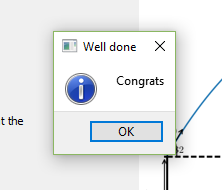
\includegraphics[width=0.5\textwidth,height=0.5\textheight,keepaspectratio]{congrats}
		\caption{Congratulation popup}
\end{figure}
The problem with this approach is that the answers to the randomly generated questions are unlikely to be a whole number, and as this approach requires the user's answer to be exactly the same as the computed answer, the user's answer would have to be over 9 decimal places long. This is an unrealistic expectation, and would cause frustration for the user. A better approach is to accept the user's answer no matter the amount of significant figures it is given to, as long as their answer is correctly rounded. 

First a method needs to be made that determines the number of significant figures that the user's answer has been given to. From the range of numbers that are used to generate the question, the correct answers will never be less than 10. This means that to calculate the number of significant figures, you can find the number of digits in the answer given by the user, and then round the actual answer to this amount of digits. This is technically not rounding a number of significant figures in every case, as sometimes the number of significant figures can be ambiguous. For example, is 40 given to 1 or 2 significant figures? So pseudocode for this
\begin{algorithm}
	\caption{Rounded answer to same significant figures as user's answer}
	\begin{algorithmic}[1]
		\State sigFig $\gets$ length(userAnswer)
		\State roundedAnswer $\gets$ round(answer, sigFig)
	\end{algorithmic}
\end{algorithm}
There is a limitation to the Python \texttt{round} function, in that it only rounds a number to a number of decimal places. An example use of the function would be \lstinline|round(1.557, 2)| would output 1.56. This is a problem as users may not round their answer to include decimal places. First the case when users give an answer with decimal places will be considered.
\begin{algorithm}
	\caption{Rounding answer to same number of decimal places in user's answer}
	\begin{algorithmic}[1]
		\If{'.' in userAnswer}
		\State dp $\gets$ length(split(userAnswer at '.'))
		\State roundedAnswer $\gets$ round(answer, dp)
		\EndIf
	\end{algorithmic}
\end{algorithm}
This algorithm will work whenever a user has a decimal place in their answer. Now for when the user does not give decimal places
\begin{algorithm}
	\caption{Rounding to same significant figures with no d.p}
	\begin{algorithmic}[1]
		\State roundedAnswer $\gets$ 17.7954
		\State roundedAnswer $\gets$ answer / 10 \Comment roundedAnswer = 1.7954
		\State roundedAnswer $\gets$ round(roundedAnswer, 1) \Comment roundedAnswer = 1.8
		\State roundedAnswer $\gets$ roundedAnswer * 10 \Comment roundedAnswer = 18
	\end{algorithmic}
\end{algorithm}
The two algorithms above can now be put together to provide code that will mark the student's answer as correct no matter the significant figures as long as it is rounded correctly. \\
\begin{lstlisting}[language=Python,caption=Answer verification]
def submit(self):
	if '.' in self.lineEdit.text():
		exponent = len(self.lineEdit.text().split('.')[1])
		rounded_answer = round(self.answer, exponent)
		print(rounded_answer)
	else:
		rounded_answer = self.answer / 10
		print(rounded_answer)
		rounded_answer = round(rounded_answer, 1)
		rounded_answer *= 10
		print(rounded_answer)
		rounded_answer = int(rounded_answer)
	if str(rounded_answer) == str(self.lineEdit.text()):
		QtWidgets.QMessageBox.information(self, "Well done", "Congrats")
		self.lineEdit.setText("")
		self.generate_question()
	else:
		QtWidgets.QMessageBox.critical(self, "Incorrect", "Unlucky m8")
		self.lineEdit.setText("")
\end{lstlisting}
This code uses the algorithm above, and gives feedback depending on the answer, either a congratulation box, or a rejection box. If the user gets the question correct, the textbox is cleared and a new question is generated. 

With the completion of this code, the initial development of the software is complete, and now testing must be done to add further developments to the software.
